\documentclass[12pt]{beamer}
\usetheme{Madrid}
\usepackage[utf8]{inputenc}
\usepackage{amsmath}
\usepackage{amsfonts}
\usepackage{amssymb}
\usepackage{graphicx}
\usepackage{float}
\usepackage{subfigure}
\author{Efrain Rojas}
\title{Atacando Captcha\\ Mediante Redes Neuronales}
%\setbeamercovered{transparent} 
%\setbeamertemplate{navigation symbols}{} 
%\logo{} 
\institute{I.I.I-UMSA} 
%\date{} 
%\subject{} 
\begin{document}

\begin{frame}
\titlepage
\end{frame}

%\begin{frame}
%\tableofcontents
%\end{frame}
%\end{frame}

\begin{frame}{Introducci\'on}
\begin{itemize}[<+->]
\item Seguridad Web
\item Procesamiento de Imagenes
\item Inteligencia Artificial
\end{itemize}
\end{frame}


\begin{frame}{Redes Neuronales}

\begin{figure}[H]
\centering
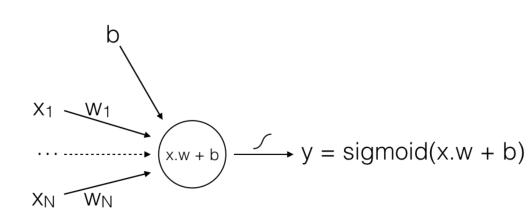
\includegraphics[scale=0.5]{2021-03-23_195019.png}
\caption{red neuronal}
\end{figure}

\end{frame}

\begin{frame}{Redes Neuronales(MLP)}

\begin{figure}[H]
\centering
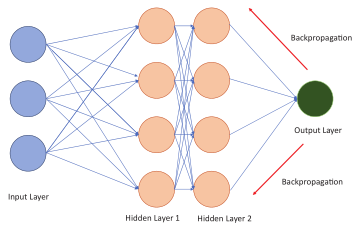
\includegraphics[scale=0.6]{2021-03-23_200337.png} 
\caption{Red neuronal multicapa}
\end{figure}

\end{frame}

\begin{frame}{Opencv}

\begin{figure}[H]
\centering
\subfigure[Opencv]{
\includegraphics[scale=1]{2021-03-23_200853.png} }
\subfigure[Operaciones basicas]{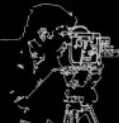
\includegraphics[scale=1]{2021-03-23_201242.png} }
\subfigure[transformaciones]{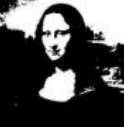
\includegraphics[scale=1]{2021-03-23_201148.png} }
\caption{Opencv y algunas Operaciones}
\end{figure}

\end{frame}

\begin{frame}{Preparando DataSet}

\end{frame}

\begin{frame}{Preprocesando datos(Imagenes)}

\end{frame}

\begin{frame}{Entrenando la red neuronal}

\end{frame}

\begin{frame}{Atacando}

\end{frame}
\end{document}